\documentclass[Japanese]{dicomopapers}
%\documentclass[Japanese,noauthor]{dicomopapers}

\usepackage[dvipdfmx]{graphicx}
\usepackage{latexsym}
\usepackage{otf}
\usepackage{url}

\def\Underline{\setbox0\hbox\bgroup\let\\\endUnderline}
\def\endUnderline{\vphantom{y}\egroup\smash{\underline{\box0}}\\}
\def\|{\verb|}

\begin{document}

% 和文表題
\title{実行可能性の検討を目的とした現実的なトポロジにおけるLow-rate DDoS攻撃のシミュレーション}
% 英文表題
\etitle{A Feasibility Study on Low-rate DDoS Attack in Realistic Topology}


% 所属ラベルの定義
\affiliate{FUN1}{公立はこだて未来大学大学院 システム情報科学研究科}
\affiliate{FUN2}{公立はこだて未来大学 システム情報科学部}

\author{\UTF{9AD9}橋 佑太}{YUTA TAKAHASHI}{FUN1}
\author{稲村 浩}{HIROSHI INAMURA}{FUN2}
\author{中村 嘉隆}{YOSHITAKA NAKAMURA}{FUN2}

\begin{abstract}
インターネット通信において広く使われているTCPは,低量分散型サービス妨害(LDDoS: Low-rate Distributed Denial of Service)攻撃によって継続的な通信妨害が可能であることが理論上と単純な環境における検証により明らかになっているが,現実のインターネットにおける実行可能性は不明である.
% DDoS攻撃フローの検知手法に関する研究は多くあるが,現在効果的な手法は確立されていない.
%  : Abstの密度では上記は不要 -- inamura
そこで本研究では,上記のネットワークの特性について現実性の高いシミュレーションを実行することで,現実のネットワークにおいて効果的なLDDoS攻撃に必要な条件・制約を明らかにし,現実のインターネットにおけるLDDoS攻撃の潜在的な標的の発見や有効な検知・緩和手法の確立を目指す.
本稿では,インターネットトポロジの特性に着目し,家庭用ブロードバンドを提供しているISPネットワークに見られる特徴を反映したトポロジを生成した.
さらに生成したトポロジにおいてLDDoS攻撃のシミュレーションを実行し,標的ボトルネックリンク帯域幅が100Mbpsの場合にTCPスループットを大きく低減させることが可能な攻撃フローの大きさを示し,今後に向けた課題を整理した.
\end{abstract}

% 表題などの出力
\maketitle

% 本文はここから始まる
% 問題と貢献
\section{はじめに}
% 一般的なDDoS
分散型サービス妨害(DDoS: Distributed Denial of Service)攻撃は,インターネットを代表する脅威のひとつである.
CDNetworksの調査では,2018年度に同社が対処したDDoS攻撃のうち,UDPフラッドやSYNフラッド等のフラッド型と呼ばれるネットワーク帯域幅攻撃が全体の半分以上の割合を占めていた\cite{cdn}.
この手法は,ボットネットから大量の攻撃トラフィックを送信することによって,標的周辺のネットワーク帯域幅や標的のCPU,メモリなどの資源を可能な限り消費し,サービスの提供を停止させるという特徴をもつ.
単純で強力な攻撃効果を生むことが可能であるが,大量の攻撃トラフィックを用いて負荷を与えるため,検知や緩和が容易である.

% LDDoSとは
Kuzmanovicらは,低量分散型サービス妨害(LDDoS: Low-rate Distributed Denial of Service)攻撃によって,TCP通信を継続的に妨害可能であることを明らかにした\cite{ldos}.
LDDoS攻撃はTCP再送信タイムアウトの仕様を利用して低い平均通信量でTCP通信を妨害することが可能であり,攻撃が完全に成功した場合,標的TCPは継続してタイムアウトを引き起こし,スループットはほぼ0まで低下する.
長さが短く高レートな矩形波のバーストトラフィックを用いて攻撃することで,攻撃トラフィックの平均通信量が一般的なフラッド型DDoS攻撃のものと比較して低量となるため,既存のDDoS攻撃トラフィックの検知手法でLDDoS攻撃トラフィックを検知することは困難である.
% 研究目的
攻撃者によってLDDoS攻撃が正確に実行された場合の脅威は大きいため,攻撃の検知についてさまざまなアプローチ\cite{cpr1}\cite{cpr2}\cite{entropy1}が検討されているが,誤検知率が高いことや,評価実験が不十分であるということが課題となっており,現在効果的な検知手法は確立されていない.
一方で,これまでにLDDoS攻撃の実例は確認されていない.
理由として,LDDoS攻撃は複数の低量トラフィックを合成して瞬時にボトルネックリンクのバッファを溢れさせる必要があるため,複雑な実ネットワークにおいては実行難易度が高く,一般的なフラッド型DDoS攻撃の方が容易に大きな効果を得られるためであることが考えられる.
しかし,DDoS攻撃はこれからも複雑化・高度化されることが予想されているため\cite{cdn},現在最も使用されている通信プロトコルであるTCPに対しステルス性の高いLDDoS攻撃が今後実行される可能性も考えられる.

効果的なLDDoS攻撃は,単純なダンベル型トポロジ(図\ref{fig:dumbbell-topology})上では実行可能であることが確認されている(詳細は2章で説明).
しかし,単純なダンベル型トポロジを現実的なネットワークに照らし合わせて考えた場合,送信ノードと攻撃ノードが同一ネットワーク内に接続されているという状況に限定されるため,LDDoS攻撃が実ネットワークにおいて真に脅威となる攻撃手法であるかは定かでない.
加えて現実のネットワークでは,以下のような様々なネットワークの特性によってパケットの損失率や遅延,ジッタが大きく変動し,正確なLDDoS攻撃フローの合成を困難にする可能性が考えられる.

\begin{itemize}
    \item ネットワークトポロジの特性
    \item ネットワークトポロジの規模
    \item 外乱トラフィックによるネットワークのリンク品質の変動
    \item ルータのキュー制御アルゴリズム
\end{itemize}

そこで本研究では,上記のネットワークの特性について現実性の高いシミュレーションを実行することで,現実のネットワークにおいて効果的なLDDoS攻撃に必要な条件・制約を明らかにし,現実のインターネットにおけるLDDoS攻撃の潜在的な標的の発見や有効な検知・緩和手法の確立を目指す.

本稿では,ネットワークトポロジの特性に着目し,以下の構成のもと,家庭用ブロードバンドにおいてLDDoS攻撃を実行する場合に必要な攻撃条件と制約を明らかにする.
2章で,背景のTCP再送信タイムアウトとLDDoS攻撃の詳細を説明する.
3章で,現実的な特性をもったトポロジでLDDoS攻撃をシミュレーションするために,家庭用ブロードバンドを提供しているISPネットワークに見られる特徴を反映したトポロジを生成する.
4章で,生成したトポロジを用いてシミュレーションを実行し,効果の高いLDDoS攻撃に必要なトラフィックの条件とその際に発生する制約について考察と議論をする.
5章で,関連研究をまとめ,さらに現実的なシミュレーションの実行のために必要な事柄と本研究の立ち位置について確認する.
6章で,まとめと今後の展望を述べる.

\section{背景}
本章では,LDDoS攻撃の原因であるTCP再送信タイムアウトと,それを利用したLDDoS攻撃の詳細に加え,実ネットワーク環境下におけるLDDoS攻撃の実行可能性について述べる.

\subsection{TCP再送信タイムアウト}

TCP通信においてパケットが送信されると,再送信タイマーがスタートする.
再送信タイマーの最大待ち時間を再送信タイムアウト(RTO:Retransmisson Time Out)と呼び,RTO以内に送信したパケットの応答が返ってこない場合,TCPは当該パケットが廃棄されたと判断し再送信する.
RTOの初期値はRFC6298\cite{rfc}により,次の式で設定される.

\begin{eqnarray}
    \label{eq:rto}
    RTO = max\{minRTO,SRTT+ \nonumber \\ max(G,4×RTTAVR)\}
\end{eqnarray}

ここで$minRTO$はRTOの最小値,$SRTT$は平滑化したラウンドトリップタイム(RTT: Round Trip Time),$G$はオペレーティングシステムに設定されているクロック粒度,$RTTAVR$はRTTの平均偏差である.
$minRTO$はRFC6298\cite{rfc}により,1秒に設定することが推奨されている.
多くの場合で(\ref{eq:rto})式の右辺では

\begin{equation}
    minRTO > SRTT + max(G,4×RTTAVR)
\end{equation}

が成り立つため,これ以降RTOの初期値は$minRTO$に設定されるものとして議論を進める.

\begin{equation}
    \label{eq:rto_1}
    RTO_1 = minRTO
\end{equation}

TCP通信において,2回以上連続して同じパケットがタイムアウトした場合,当該パケットが再送なく正常に応答を返すまでタイムアウトごとにRTOの値を2倍ずつ増加させていく.
$i$回連続でタイムアウトしたパケットのRTOの値を$RTO_i$と表すとこの値は以下の(\ref{eq:rto_i})式により設定される.
ただし,RTOの値は60秒以上の上限値を持つように制限されている.

\begin{equation}
    \label{eq:rto_i}
    RTO_i = 2RTO_{i-1}
\end{equation}

当該パケットの送信と応答が成功した場合,(\ref{eq:rto_1})式によりRTOは$minRTO$に再設定される.
このアルゴリズムはKarnのアルゴリズムと呼ばれ,ほとんどのTCPで実装されているが,$RTO_i$が$minRTO$に依存して一意に決定される単純な仕様が,LDDoS攻撃に利用される.
攻撃者は$minRTO$の間隔で標的コネクションを輻輳させることにより,低い平均通信量で標的のTCP通信は継続してタイムアウトを引き起こし,スループットを低下させることが可能である.

\subsection{LDDoS攻撃}
LDDoS攻撃は短いバーストトラフィックと無通信が一定の周期で繰り返される矩形波状のLDDoS攻撃フロー(図\ref{fig:LDoS-flow})を複数の攻撃ノードから送信し,標的TCPパケットがボトルネックリンクを流れるわずかな時間のみ輻輳を繰り返し発生させ,低い平均通信量でTCP通信を妨害することが可能な攻撃手法である\cite{ldos}.

\subsubsection{LDDoS攻撃フローのモデル化}
1つの攻撃ノードが送信するLDDoS攻撃フローをバースト間隔$T_a$,バースト幅$T_b$,バーストレート$R_b$,攻撃開始時間$s$により定義する(図\ref{fig:LDoS-flow}).

\begin{figure}[htbp]
    \begin{center}
        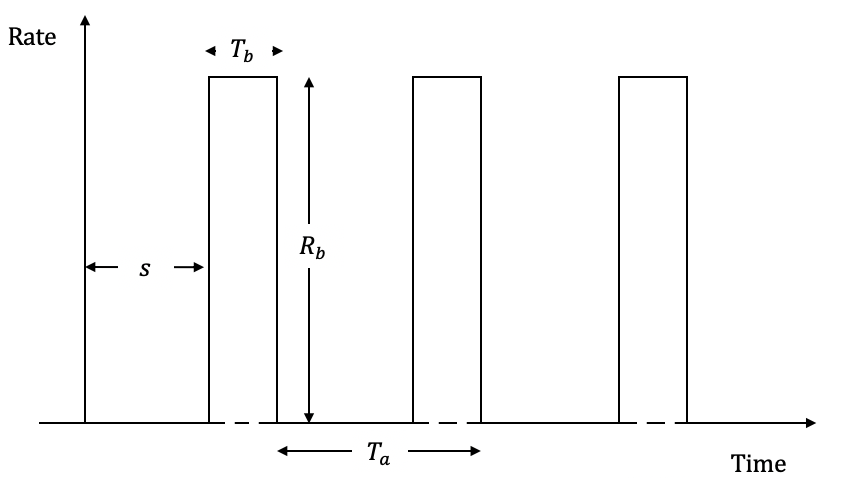
\includegraphics[clip,width=8.0cm]{images/LDoS-flow.png}
        \caption{LDDoS攻撃の単一フロー 複数のフローを合成することによりボトルネックリンクのバッファを溢れさせる}
        \label{fig:LDoS-flow}
    \end{center}
\end{figure}

複数のフローがボトルネックリンク上で合成されたLDDoS攻撃フローのバースト間隔を$T_a^+$,バースト幅を$T_b^+$,バーストレートを$R_b^+$と定義する(図\ref{fig:lddos-example}).
文献\cite{cpr1}では,更に詳細にモデル化されている.

\begin{figure}[tb]
    \begin{center}
        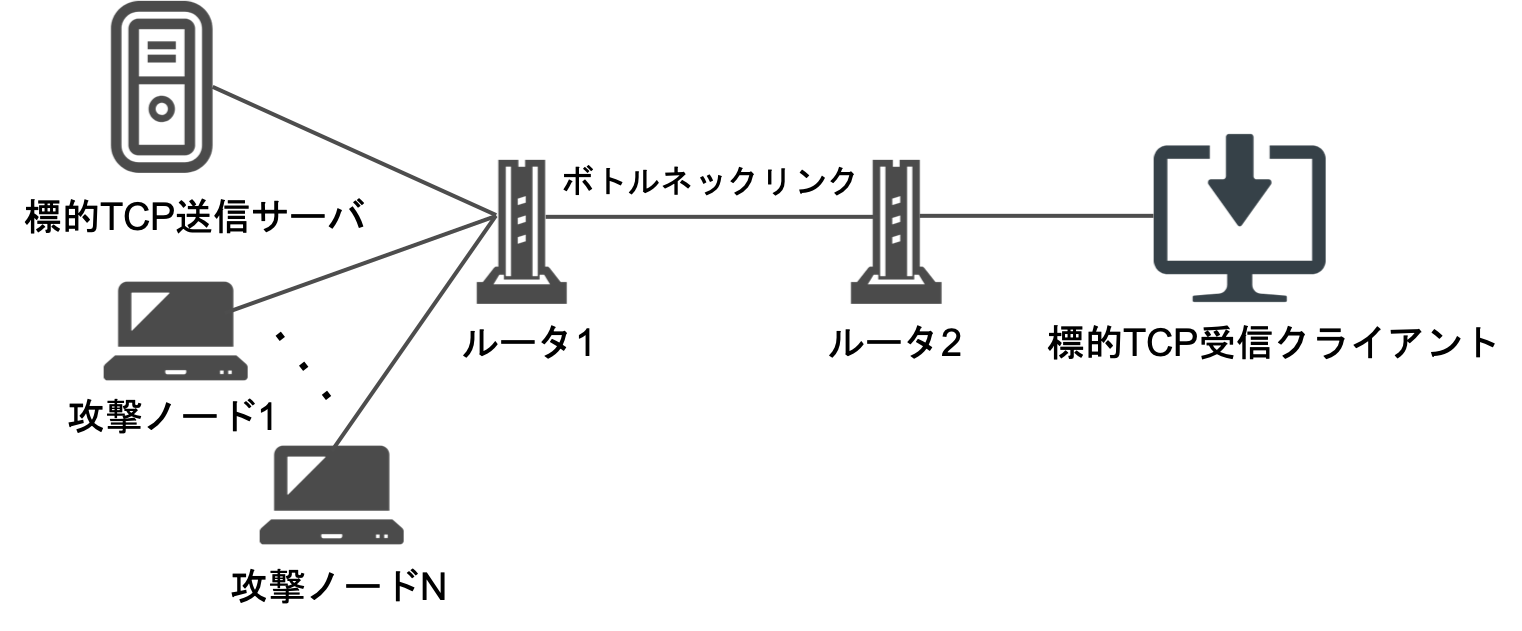
\includegraphics[clip,width=8.0cm]{images/dumbbell.png}
        \caption{効果的なLDDoS攻撃が可能なダンベル型トポロジ 標的TCPの送信ノードとすべての攻撃ノードがルータ1に接続されており,ルータ1のバッファを溢れさせることにより,送信ノードから受信ノードに向けたTCPパケットを妨害する.}
        \label{fig:dumbbell-topology}
    \end{center}
\end{figure}

\begin{figure*}[t]
    \begin{center}
      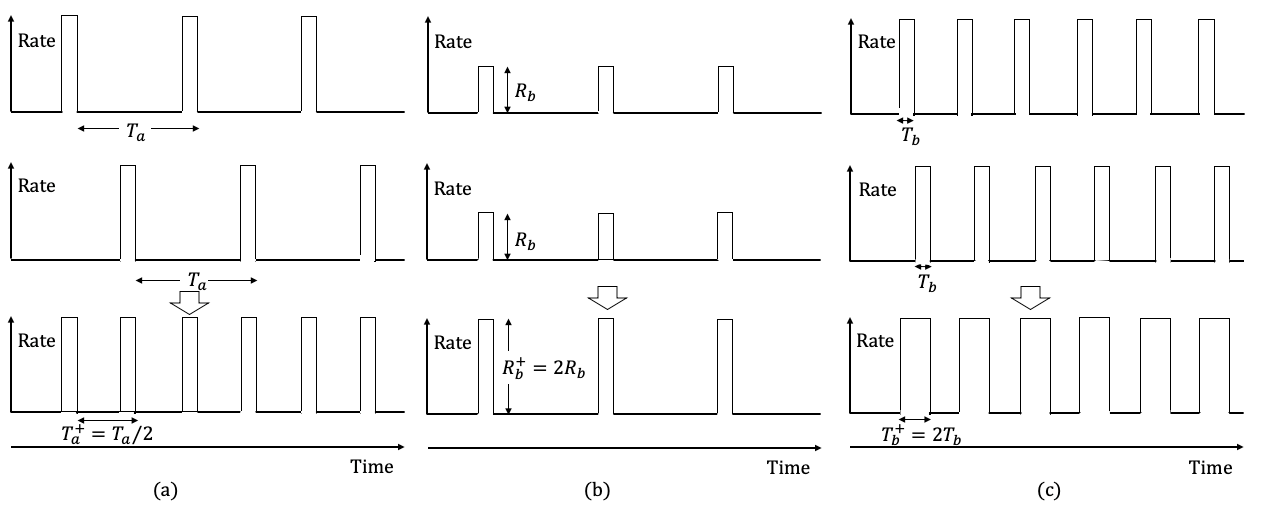
\includegraphics[clip,width=17.0cm]{images/lddos-example.png}
      \caption{LDDoS攻撃フローの合成(a)バースト間隔,(b)バーストレート (c)バースト幅 
      (文献\cite{cpr1}図3を参考に作成)}
      \label{fig:lddos-example}
    \end{center}
\end{figure*}

\subsubsection{効果的なLDDoS攻撃}
LDDoS攻撃は,$T_a^+$をminRTOと等しい長さ,$T_b^+$を200msから300msの長さ,$R_b^+$をボトルネックリンクのバッファを十分に満たす大きさに設定した場合に最も大きな効果を生み,標的のTCPスループットをほぼ0まで低下可能であることが示されている\cite{ldos}\cite{practical-ldos-defense}.

ボトルネックリンク上で上記パラメータを満たすLDDoS攻撃フローを生成できた場合,1回目の合成バーストトラフィックにより,ボトルネックリンクのバッファが溢れ,標的のTCPのパケットが喪失する.
次に,標的TCPは(\ref{eq:rto_1})式により,minRTOだけ再送信タイムアウトを待ったあと喪失したパケットを再送信する.
このとき,タイミングを合わせて攻撃フローを繰り返し送信し,合成バーストトラフィックを生成して攻撃を継続することで,再びボトルネックリンクのバッファが溢れるため標的TCPのパケットが喪失する.
その後も標的TCPのminRTOと同じバースト間隔でバーストトラフィックを送信を続けることで,標的TCPの送信ノードのRTOが(\ref{eq:rto_i})式により,minRTOの倍数の値を取り続けるため,バーストトラフィックと再送信のタイミングが重なり,通信が抑止された状態が継続される.

効果的なLDDoS攻撃を検証している多くの研究(シミュレーション\cite{ldos}\cite{cpr2}\cite{lddos-flow-aggregation},実証実験\cite{mine-wip-paper})では,単純なダンベル型トポロジ(図\ref{fig:dumbbell-topology})を用いており,現実のインターネットのように複雑な環境においても同様に実行可能であるかは明らかではない.

% 3章
\section{シミュレーション環境の設定}
本章では,家庭用ブロードバンドを提供しているISPネットワークに見られる特徴を反映したシミュレーション環境の設定について説明する.
シミュレーションにはネットワークシミュレータns-3\cite{ns-3}を使用する.
以下の特性を設定し,図\ref{fig:generated-topology}のトポロジを生成した.
図\ref{fig:generated-topology}中のノードの説明を表\ref{tab:node-description}に示す.

\begin{figure}[tb]
    \begin{center}
        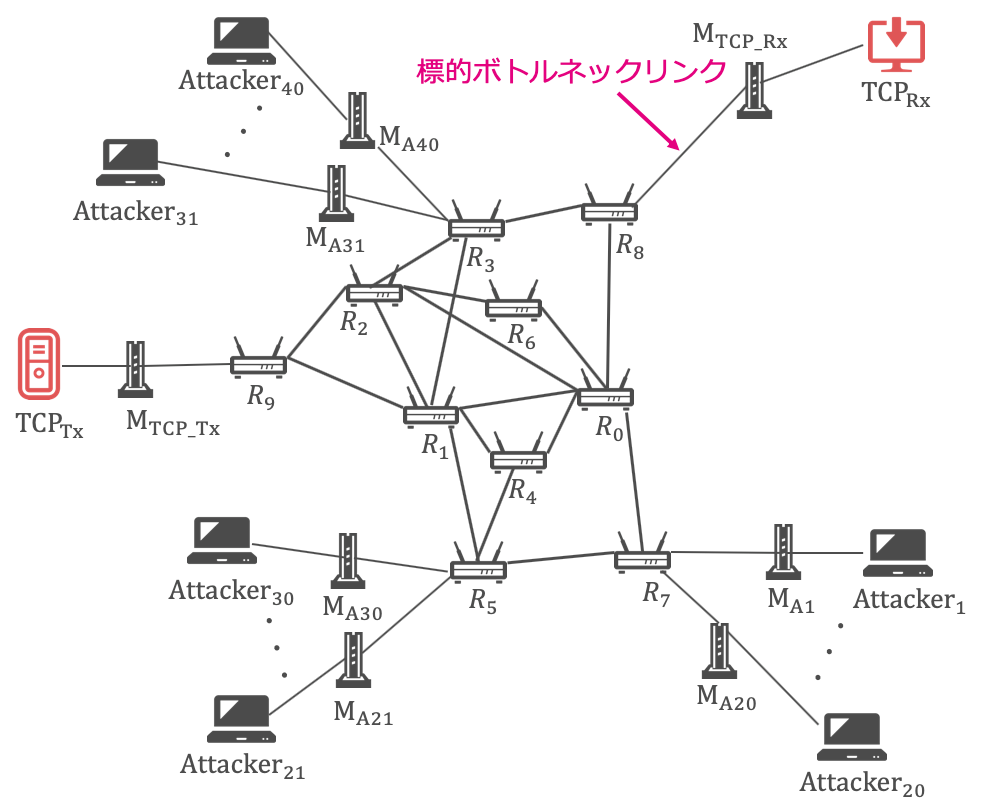
\includegraphics[clip,width=8.0cm]{images/generated-topology-big.png}
        \caption{生成したトポロジ}
        \label{fig:generated-topology}
    \end{center}
\end{figure}

\begin{table}[htbp]
    \caption{ノードの説明}
    \label{tab:node-description}
    \begin{center}
        \scalebox{0.80}[1.0]{
            \begin{tabular}{ll}
                \hline
                \multicolumn{1}{c}{ノード}             & \multicolumn{1}{c}{説明}        \\ \hline
                $R_{0} \cdots R_{9}$                & バックボーンルータ0$\cdots$バックボーンルータ9  \\
                $TCP_{Tx}$                          & 標的TCP送信サーバ                    \\
                $TCP_{Rx}$                          & 標的TCP受信クライアント                 \\
                $Attacker_{1} \cdots Attacker_{40}$ & 攻撃ノード1$\cdots$攻撃ノード40         \\
                $M_{TCP_Tx}$                        & 標的TCP送信サーバのモデム                \\
                $M_{TCP_Rx}$                        & 標的TCP受信クライアントのモデム             \\
                $M_{A1} \cdots M_{A40}$             & 攻撃ノード1$\cdots$攻撃ノード40それぞれのモデム \\ \hline
            \end{tabular}
        }
    \end{center}
\end{table}

\subsection{トポロジの構成}
BarabasiとAlbertによって
現実のバックボーンネットワークにはスケールフリー性(次数分布のべき乗則)が見出されており,
BAモデルとして知られている\cite{ba-model}.
Kongらは数多く存在するDDoS攻撃検知手法の現実的な有効性を実証するためには,BAモデルのトポロジを用いたDDoS攻撃のシミュレーションが有効であると提案している\cite{random-flow-ddos}.

そこで,上記を参考にns-3でサポートされているトポロジジェネレータBRITE\cite{brite}を用いてBAモデルのトポロジを生成し,シミュレーションを実行する.
表\ref{tab:brite-param}にトポロジの生成使用するBRITEの設定パラメータを示す.
現実のISPは複数のASによって構成されている\cite{realistic-topologies}が,複雑性を徐々に上げていくため今回は複数のASを考慮せず,すべてのノードを1つのAS内に配置するRouter BAモデルで生成した.
今回のシミュレーションでは,BRITEで生成した10個のノード($R_{0} \cdots R_{9}$)をISPのASトポロジ一つを構成するバックボーンルータと想定する.
次に標的TCP送信サーバ($TCP_{Tx}$ )1台,標的TCP受信クライアント($TCP_{Rx}$)1台,攻撃ノード40台($Attacker_{1} \cdots Attacker_{40}$)をそれぞれの各モデムノード($M_{TCP_Tx}$,$M_{TCP_Rx}$,$M_{A1} \cdots M_{A40}$)と接続し,モデムノードをバックボーンルータに接続した.

\begin{table}[htbp]
    \caption{BRITE設定パラメータ}
    \label{tab:brite-param}
    \begin{center}
        \scalebox{0.80}[1.0]{
            \begin{tabular}{lll}
                \hline
                \multicolumn{1}{c}{パラメータ(意味)} & \multicolumn{1}{c}{設定値} & \multicolumn{1}{c}{備考} \\ \hline
                Name (モデル)                    & 2                       & Router BA model        \\
                N (ノード数)                      & 10                      &                        \\
                HS (主平面の大きさ)                  & 1,000                   & デフォルト値                 \\
                LS (内面の大きさ)                   & 100                     & デフォルト値                 \\
                NodePlacement (ノード配置方法)       & 1                       & ランダム                   \\
                m (link/node)                 & 2                       &                        \\
                BWDist (帯域幅の割当分布)             & 1                       & 一定(すべてBWMinに固定)        \\
                BWMin (最小帯域幅)                 & 2,500                   & 2.5Gbps                \\
                BWMax (最大帯域幅)                 & 2,500                   & BWDistが一定のため無効         \\ \hline
            \end{tabular}
        }
    \end{center}
\end{table}

\subsection{リンクパラメータ・ボトルネックリンクの位置}
北米とヨーロッパの主要ISPを対象にしたDischingerらの家庭用ブロードバンドネットワークの調査によって,住宅ネットワークのバックボーンルータと家庭に設置されたモデムを繋ぐブロードバンドリンク(ラストマイル)がボトルネックリンクになっていることが明らかとなった\cite{broadband-characterizing}.
これを参考に,インターネットトポロジと攻撃ノードが接続されたモデムノードを繋ぐリンクがボトルネックとなるように帯域幅とRTTを設定する.

$R_{0} \cdots R_{9}$を結ぶ各リンクの帯域幅は,文献\cite{internet-backbone}を参考に2.5Gbps,バックボーントポロジのRTTはごく僅かな値として0.75msを設定した.
その他のリンクの帯域幅とRTTは表\ref{tab:link-param}の値を設定した.
標的TCP受信クライアントと攻撃ノードは家庭用ブロードバンドに接続されていると仮定し,それらが接続されているモデムのブロードバンドリンクの下り帯域幅を100Mbps,上り帯域幅を10Mbpsに設定した.
文献\cite{mine-wip-paper}において我々はIoT端末のRaspberry Piを用いて$R_{b}=$10MbpsのLDDoS攻撃フローを生成できたことから,上り帯域幅の設定は現実的な値として考えられる数値であるといえる.
標的TCP送信サーバは他ISPのサービス事業者用のネットワークから接続されていると仮定し,帯域幅を1,000Mbpsに設定した.
RTTの現実性は今回のシミュレーションで考慮せず,すべての攻撃ノードが適切に攻撃フローを合成できるようにボトルネックリンクルータ$R_{8}$までのRTTをほぼ等しく設定した.

\begin{table}[tb]
    \caption{リンクパラメータ}
    \label{tab:link-param}
    \begin{center}
        \scalebox{0.80}[1.0]{
            \begin{tabular}{lll}
                \hline
                \multicolumn{1}{c}{リンク}                           & \multicolumn{1}{c}{帯域幅(Mbps)} & \multicolumn{1}{c}{RTT (ms)} \\ \hline
                $TCP_{Tx}$ to $M_{TCP_Tx}$                        & 1,000                         & 1                            \\
                $M_{TCP_Tx}$ to $R_{9}$                           & 100                           & 10                           \\
                $TCP_{Rx}$ to $M_{TCP_Rx}$                        & 1,000                         & 1                            \\
                $M_{TCP_Rx}$ to $R_{8}$ (標的ボトルネックリンク)             & 100                           & 5                            \\
                $Attacker_{i}$ to $M_{Ai} (i = 1, 2, \cdots, 40)$ & 1,000                         & 1                            \\
                $M_{A1} \cdots M_{A20}$ to $R_{7}$                & 10                            & 10                           \\
                $M_{A21} \cdots M_{A30}$ to $R_{5}$               & 10                            & 10                           \\
                $M_{A31} \cdots M_{A40}$ to $R_{3}$               & 10                            & 10                           \\ \hline
            \end{tabular}
        }
    \end{center}
\end{table}

\subsection{ルータバッファ}
$R_{0} \cdots R_{9}$の各リンクのネットワークデバイスにはBRITEの初期値である100pktsのドロップテールキューを設定した.

\subsection{LDDoS攻撃に必要な前提条件}
図\ref{fig:generated-topology}のトポロジでLDDoS攻撃を実行するために必要な前提条件を整理する.

\begin{enumerate}
    \item 攻撃者は$Attacker_{1} \cdots Attacker_{40}$を自由に操作可能である.
    \item 攻撃者は$Attacker_{1} \cdots Attacker_{40}$と$R_{8}$間のRTTを計測し,それぞれの攻撃開始時間を指定できる.
    \item $Attacker_{1} \cdots Attacker_{40}$と$R_{8}$間のRTTが安定しており大きなジッタは発生しない.
    \item $M_{A1} \cdots M_{A40}$に$Attacker_{1} \cdots Attacker_{40}$以外のノードが接続されていた場合,それらのノードは攻撃フローを送信している間は通信を行わない.
    \item 攻撃者は$TCP_{Tx}$のminRTOを特定している.(今回は1秒に設定)
\end{enumerate}

以上が満たされたと仮定してシミュレーションを実行する.

% シミュレーション
\section{シミュレーション実験}
\subsection{効果的なLDDoS攻撃に必要なバーストレートと攻撃ノード数の推定}
3章で生成した家庭用ブロードバンドネットワークの特性を設定したトポロジにおいて,効果的なLDDoS攻撃に必要なバーストレートと攻撃ノード数をシミュレーションにより検証する.
標的TCPスループットを1割未満に妨害することが可能なバーストレートの大きさを明らかにするために,ボトルネックリンクルータである$R_{8}$のバッファを100pktsと1,000pktsに設定したそれぞれの場合について,以下のシミュレーションを実行する.

$TCP_{Tx}$は$TCP_{Rx}$へ200MBのデータを60秒間可能な限りBulk Sendで送信し,その平均正規化スループットを計測する.
攻撃ノード1台当たり$T_{a} = 1.0s$,$T_{b} = 250ms$,$R_{b}=10Mbps$の攻撃フローを$TCP_{Rx}$に送信し,$TCP_{Tx}$のTCPを妨害する.
シミュレーションは計40回実行する.
1回のシミュレーションごとに,$Attacker_{1}$から$Attacker_{40}$を1台ずつ参加させ,攻撃に参加するノードはすべて同時刻に攻撃を開始する.
今回はすべての攻撃ノードからボトルネックリンクルータ$R_{8}$までのRTTがほぼ等しくなるように設定したため,$R_{8}$で合成された攻撃フローの合計パラメータは$T_{a}^+ = 1.0s$,$T_{b}^+ = 250ms$,$R_{b}^+=10, 20, \cdots, 400Mbps$となる.

\subsection{実験結果}
シミュレーションの結果を図\ref{fig:exp01-result}に示す.
標的TCPの平均正規化スループットを1割未満に低下させるために最低限必要な合計バーストレート$R_{b}^+$は,ボトルネックリンクルータ$R_{8}$のバッファが100pktsの場合は約270Mbps,1,000pktsの場合は約340Mbpsという結果が得られた.
よって,家庭用ブロードバンドの特性を設定したトポロジにおいて,攻撃者が3.4節の前提条件を満たすことができた場合,効果的なLDDoS攻撃が実行可能であることが明らかになった.

\begin{figure}[tb]
    \begin{center}
        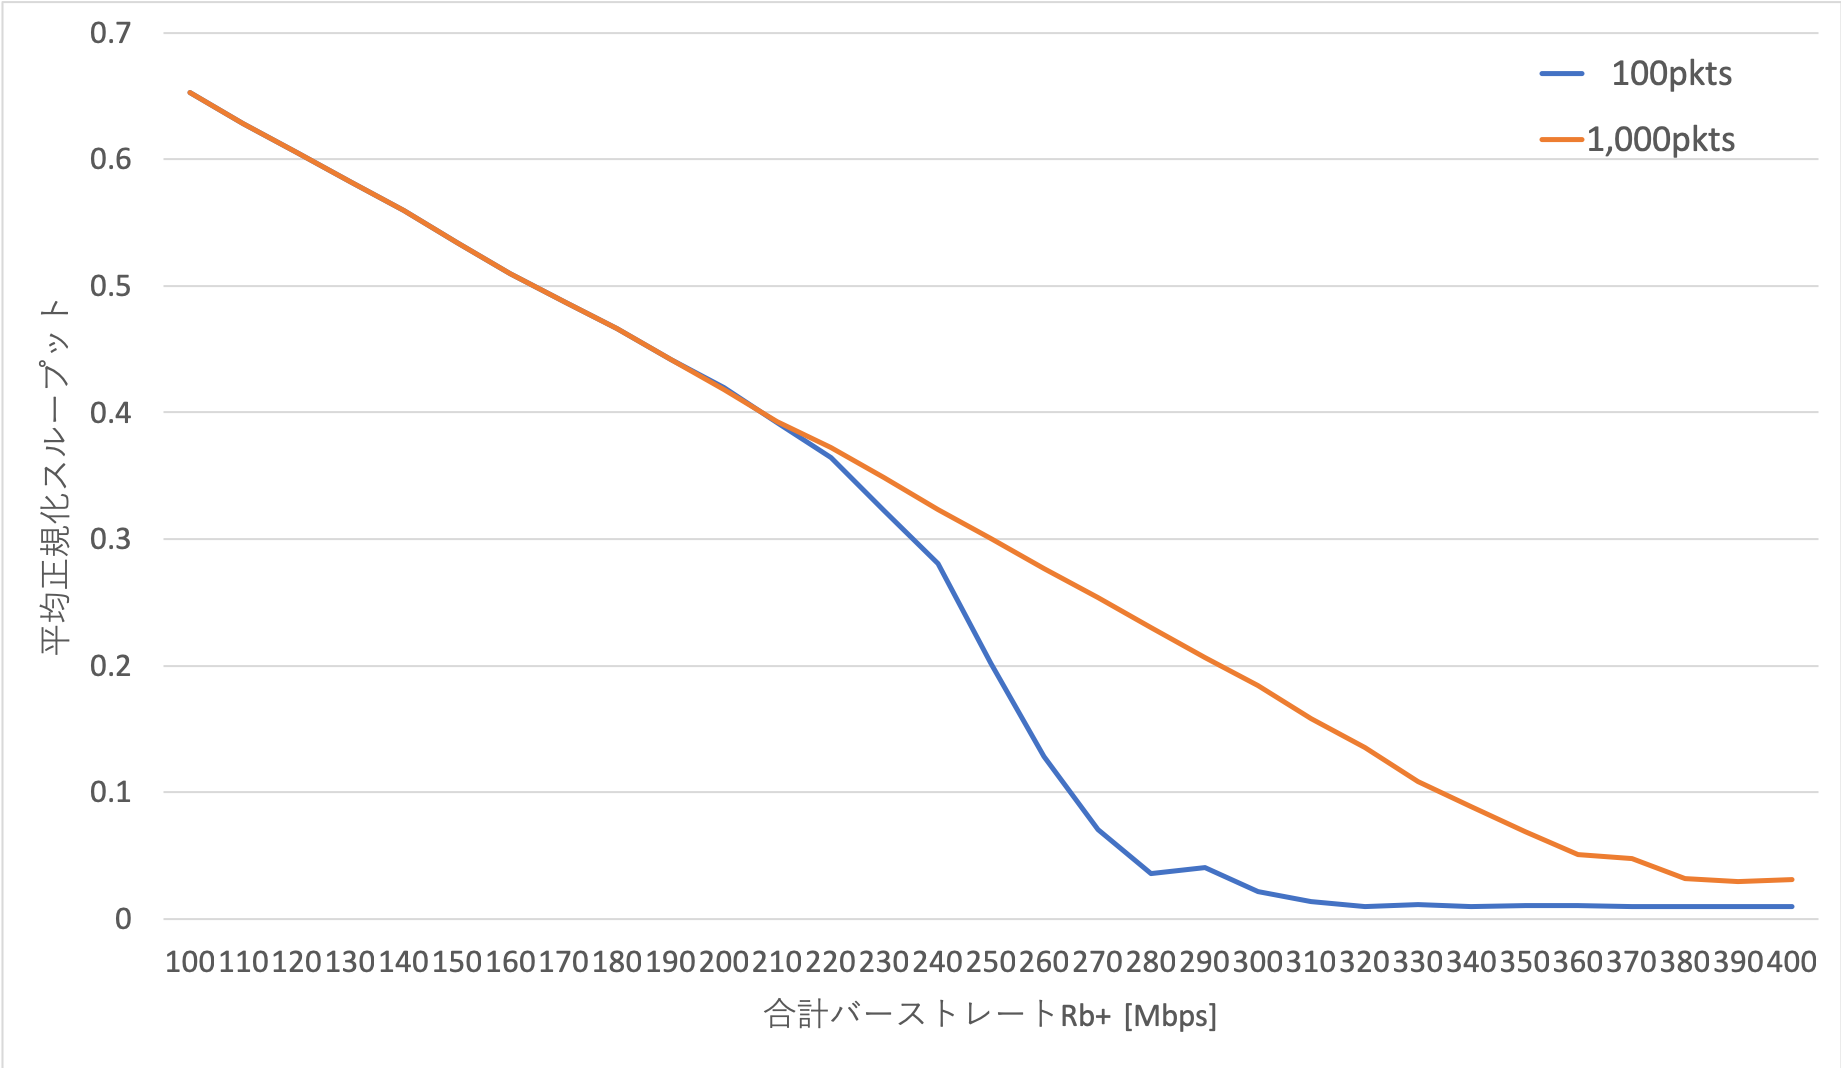
\includegraphics[clip,width=8.5cm]{images/exp01-result.png}
        \caption{ボトルネックリンクルータ$R_{8}$のバッファとバーストレート$R_{b}^+$の増加による標的TCPの平均正規化スループットの推移}
        \label{fig:exp01-result}
    \end{center}
\end{figure}

\subsection{考察}
本節では,効果的なLDDoS攻撃に必要な条件と制約,現実性について考察する.

\subsubsection{攻撃に必要な条件と制約}
攻撃ノードの配置に関する制約と現実性について考察する.
一般的なバックボーンリンクの使用率は10\%から30\%であると文献\cite{sizing-router-buffers}で述べられている.
今回のトポロジでバックボーンリンク全体の帯域幅が他の一定的なトラフィックによって30\%使用された場合,残りの使用可能帯域幅は1.75Gbpsとなる.
よって$R_{b}^+$が1.75Gbps未満の場合,すべての攻撃フローが同じリンク経路を流れたとしてもリンクが溢れることはないため,攻撃フローが損失されないことから,攻撃ノードの配置を考慮しなくても効果的な攻撃を実現できるといえる.
したがって,今回のシミュレーションにおいて効果的なLDDoS攻撃を実行するために必要な条件は,ボットネット環境を構築する際に最低限340Mbpsの帯域幅を確保することであるといえる.
このときに攻撃ノードの配置に関する制約はない.
一方で,標的ボトルネックリンクの帯域幅が高く,必要なバーストレート$R_{b}^+$が1.75Gbps以上必要となる場合に攻撃フローが一部のリンクに集中してしまうとロスが発生するため,攻撃ノードの配置に制約が生まれることが考えられる.
この制約について一般化し,明らかにすることは今後の課題となる.

攻撃ノードの配置については,標的ボトルネックリンクと同じAS内にすべての攻撃ノードを構築することは現実的ではない.
より現実的なシミュレーションにするために複数のASトポロジを考慮し,トポロジの規模拡大と攻撃ノードを複数のASトポロジに分散した際に発生する制約を明らかにすることが課題として挙げられる.

\subsubsection{ボトルネックリンクルータのバッファによる攻撃効果の低減}
図\ref{fig:exp01-result}の結果から,標的ボトルネックリンク帯域幅の2倍から3倍のバーストレートの攻撃フローに対して,ルータのバッファが大きいほど,スループットの損失率を大きく低減できることがわかった.
バーストレートが標的ボトルネックリンクの4倍以上の大きさである$R_{b}^+=400Mbps$の場合,ルータのバッファサイズによる平均正規化スループットに変化はほとんど見られないため,リンクに対して過剰なバーストレートに対する検知精度を高め,検知が難しいそれ以下のバーストレートに対してはルータのバッファサイズを多く確保することにより,攻撃の検知と緩和を両立できる可能性があると考える.

\section{関連研究}
% さらに現実的なシミュレーションの実行のために必要な事柄
% On realistic network topologies for simulation\cite{realistic-topologies} について 
Heckmannらはネットワークトポロジを比較するための類似性メトリクスを提示し,それに基づいて現実のISP(DFN,AT\&T)に類似性が高いトポロジをBRITEなどのトポロジジェネレータで生成するために必要なパラメータを導き出した\cite{realistic-topologies}.
これを使用することで現実性の高いトポロジを生成できるため,今後これらのパラメータを活用していく.

% 現実的なLDDoS攻撃の実行可能性について関連した研究の紹介と本研究の立ち位置
Fengらはデータセンターネットワーク(DCN: Data Center Network)におけるLDDoS攻撃の実行可能を検証した\cite{dcn-shrew}.
DCNは高帯域幅,低遅延で安定しており,トポロジの特性も限られているいるため,悪意のあるテナントがLDDoS攻撃によって同じネットワークリソースを共有している他のテナントのTCP通信を妨害できる危険性があった.
24台の物理サーバに48台のVMを構築して再現したDCNのテスト環境を用いてLDDoS攻撃を検証した結果,TCPスループット損失率が最大83\%まで上昇したことからDCNにおいてLDDoS攻撃が有効であることが示された.
この研究はLDDoS攻撃の実行可能性を議論している点で関連しているが,本研究はさらに一般的なインターネット上における実行可能性を明らかにすることが目的である.

\section{おわりに}
\subsection{まとめ}
本稿では,家庭用ブロードバンドの特徴を設定したトポロジを用いてLDDoS攻撃をシミュレーションし,ボトルネックリンクの帯域幅が100Mbpsの場合,合計バーストレートが270Mbpsから340MbpsのLDDoS攻撃フローを生成することで,標的TCPスループットを1割以下に低減させることが可能であることを確認した.
さらに,攻撃に必要な条件と制約やボトルネックリンクルータのバッファによる攻撃効果の低減からLDDoS攻撃の検知・緩和について考察した.

\subsection{今後の展望}
現実のインターネットにおけるLDDoS攻撃を実行可能性をさらに詳しく検討するために,今回のシミュレーションの課題とアプローチについてまとめる.
1つ目はトポロジのモデルである.
今回のシミュレーションではASトポロジについて考慮できなかったため,ASトポロジとRouterトポロジを組み合わせ,遅延や帯域幅について現実のトポロジに近似したトポロジモデルを構築する必要がある.
2つ目はトラフィックモデルである.
文献\cite{random-flow-ddos}のように,統計的モデルを使用した現実的なバックグラウンドトラフィックを生成し,ジッタによるRTTの変動が大きい環境におけるLDDoS攻撃の実行可能性について検証する必要がある.
3つ目はルータのキュー制御アルゴリズムである.
今回のシミュレーションではすべてのルータにDroptailを設定したが,REDなどのキュー制御アルゴリズムもトポロジモデルやトラフィックモデルと同時に考慮する必要がある.
これらの他に,攻撃者が実ネットワークにおいて,3.4節で設定したLDDoS攻撃に必要な前提条件を満たすことができるのかについても検証する必要がある.

\begin{thebibliography}{99}
    \bibitem{cdn} 株式会社シーディーネットワークス・ジャパン:2018年度、DDoS攻撃の動向と今後の見通し,CDNetworksセキュリティレポート(オンライン),\urlj{https://engage.cdnetworks.co.jp/LP\_WP36} \refdatej{2019-04-19}
    \bibitem{ldos} Kuzmanovic,A. and Knightly,E. W.:Low-rate TCP-targeted Denial of Service Attacks and Counter Strategies,IEEE/ACM Transactions on Networking,Vol.14,No.4,pp.683-696 (2006).
    \bibitem{cpr1} Zhang,C.,Cai,Z.,Chen,W.,et al.:Flow level detection and filtering of low-rate DDoS,Computer Networks,Vol.56,No.15,pp.3417-3431 (2012).
    \bibitem{cpr2} Kieu,M. V.,Nguyen,D. T.,and Nguyen,T. T.:Using CPR Metric to Detect and Filter Low-Rate DDoS Flows,Proceedings of the Eighth International Symposium on Information and Communication Technology. ACM,pp.325-332 (2017).
    \bibitem{entropy1} Jadhav,P. N. and Patil,B. M.:Low-rate DDOS Attack Detection using Optimal Objective Entropy Method,International Journal of Computer Applications,Vol.78,No.3,pp.33–38 (2013).
    \bibitem{rfc} Paxson,V.,Allman,M.,Chu,J.,et al.:Computing TCP's Retransmission Timer,Internet RFC 6298(オンライン),\urlj{https://tools.ietf.org/html/rfc6298} \refdatej{2019-05-01}.
    \bibitem{practical-ldos-defense} Efstathopoulos,P.:Practical study of a defense against low-rate TCP-targeted DoS attack,2009 International Conference for Internet Technology and Secured Transactions,(ICITST). IEEE,pp.1-6 (2009).
    \bibitem{lddos-flow-aggregation} Zhijun,W.,Lan,M.,Minghua,W.,et al.:Research on Time Synchronization and Flow Aggregation in LDDoS Attack Based on Cross-correlation,2012 IEEE 11th International Conference on Trust,Security and Privacy in Computing and Communications. IEEE,pp.25-32 (2012).
    \bibitem{mine-wip-paper} \UTF{9AD9}橋 佑太,稲村 浩,中村 嘉隆:実ネットワーク環境下におけるLDDoS攻撃の検証,研究報告モバイルコンピューティングとパーベイシブシステム(MBL),Vol.2018-MBL-89,No.8,pp.1-7 (2018).
    \bibitem{ns-3} ns-3 | a discrete-event network simulator for internet systems,\urlj{https://www.nsnam.org/}\refdatej{2019-05-01}.
    \bibitem{ba-model} Barab{\'a}si,A.L. and Albert,R.:Emergence of scaling in random networks,science,Vol.286,No.5439,pp.509-512 (1999).
    \bibitem{random-flow-ddos} Kong,J.,Mirza,M.,Shu,J.,et al.:Random flow network modeling and simulations for DDoS attack mitigation,IEEE International Conference on Communications,2003. ICC'03.. IEEE,Vol.1,pp.487-491 (2003).
    \bibitem{brite} Medina,A.,Lakhina,A.,Matta,I.,et al.:BRITE:An approach to universal topology generation,MASCOTS 2001,Proceedings Ninth International Symposium on Modeling,Analysis and Simulation of Computer and Telecommunication Systems. IEEE,pp.346-353 (2001).
    \bibitem{realistic-topologies} Heckmann,O.,Piringer,M.,Schmitt,J.,et al.:On realistic network topologies for simulation,Proceedings of the ACM SIGCOMM workshop on Models,methods and tools for reproducible network research. ACM,pp.28-32 (2003).
    \bibitem{broadband-characterizing} Dischinger,M.,Haeberlen,A.,Gummadi,K. P.,et al.:Characterizing residential broadband networks,Internet measurement conference,Vol.7,pp.43-56 (2007).
    \bibitem{internet-backbone} Fraleigh,C. J.:Provisioning Internet Backbone Networks to Support Latency Sensitive Applications. PhD thesis,Stanford University (2002).
    \bibitem{sizing-router-buffers} Appenzeller,G.,Keslassy,I.,and McKeown,N.:Sizing router buffers,ACM,Vol.34,No.4,pp.281-292 (2004).
    \bibitem{dcn-shrew} Feng,Z.,Bai,B.,Zhao,B.,et al.:Shrew Attack in Cloud Data Center Networks,2011 Seventh International Conference on Mobile Ad-hoc and Sensor Networks. IEEE,pp.441–445 (2011).
\end{thebibliography}

\end{document}
